\documentclass[11pt]{beamer}
\usepackage[utf8]{inputenc}
\usepackage[T1]{fontenc}
\usepackage{amsmath}
\usepackage{amsfonts}
\usepackage{amssymb}

\usetheme{default}
\usepackage{graphicx}
\begin{document}
    \author{A. Zelenaya \inst{1}, M. Zelenyi \inst{1,2}, A.A.Turinge \inst{1},  V.G. Nedorezov \inst{1}}
    \title{Chemical composition analysis for X-ray transport container scans. }
    %\subtitle{}
    % \logo{}
    \institute[INR]{
        \inst{1} Institute for Nuclear Research RAS \and
        \inst{2} Moscow Institute of Physics and Technology (SU)
    }
    \date{October 10, 2018}
%    \subject{Moscow}
    %\setbeamercovered{transparent}
    %\setbeamertemplate{navigation symbols}{}
    \frame[plain]{\maketitle}
    
    \begin{frame}
        \frametitle{Target}
    \end{frame}
    \begin{frame}
    \frametitle{Methodology: Gamma ray attenuation}
    \begin{columns}
        \begin{column}{0.8\textwidth}
            $$
            T(E_0, t, z) = \frac{\int \limits_0^{E_0} S(E_0, E) \exp(-\mu(E,z)\times t)~dE)}{\int \limits_0^{E_0} S(E_0, E)~dE}
            $$
               \includegraphics[width=1\textwidth]{figures/Attenuation.pdf}
        \end{column}
    \vline~
        \begin{column}{0.4\textwidth} 
            $T$ -  transmittance\\
            $S(E_0, E)$ - response function\\
            $\mu(E,z)$ - attenuation coefficient\\
            $t$ -  optical thickness\\
            $E_0$ -  up-limit energy of bremsstrahlung\\
            $E$ - energy of gamma ray\\
        \end{column}
    \end{columns}  
\end{frame}

\begin{frame}
    \frametitle{Methodology: Exist solution}
    \begin{block}{Dual energy method}
        
        $$
        F(z) = \frac{|t(E^{(1)}_0,z) - t(E^{(2)}_0,z)|}{t(E^{(1)}_0,z)} \to min
        $$
    \end{block}

    \begin{block}{Disadvantages}
        \begin{itemize}
            содержимое...
        \end{itemize}
    \end{block}
%    \begin{columns}
%        \begin{column}{0.9\textwidth}
%
%        \end{column}
%         \begin{column}{0.4\textwidth}
%           
%            
%        \end{column}
%    \end{columns} 
\end{frame}
%-------------Экспериментальная часть--------------------------
\begin{frame}
    \frametitle{Experiment: Energy resolution of detector}
    \begin{columns}
        \begin{column}{0.5\textwidth}
            
            \includegraphics[width=1\textwidth]{figures/setup1.png}
        \end{column}
                \begin{column}{0.5\textwidth}
            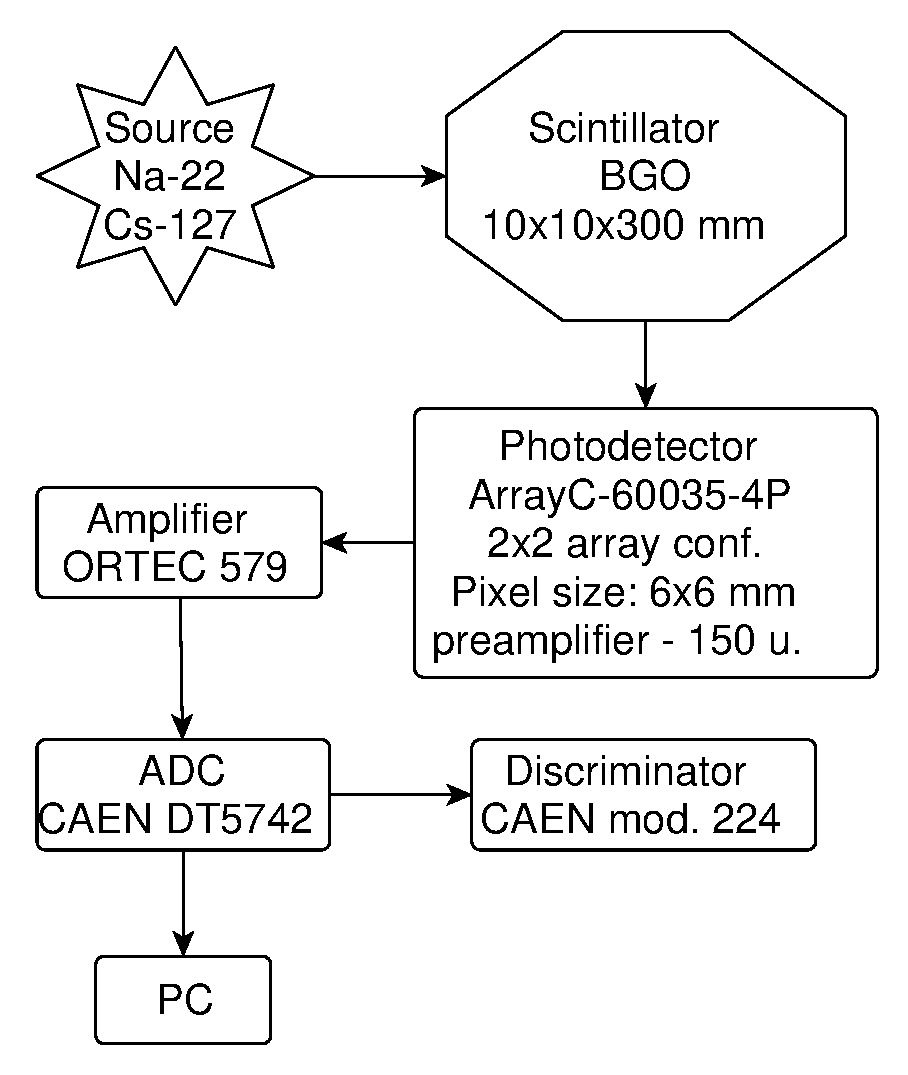
\includegraphics[width=1\textwidth]{figures/yed.pdf}
        \end{column}
    \end{columns}  
\end{frame}

\begin{frame}
    \frametitle{Experiment: Energy resolution of detector}
    \begin{columns}
        \begin{column}{0.5\textwidth}
            $^{22}Na$ --- $0.511 MeV$\\
            \includegraphics[width=1\textwidth]{figures/setup3.png}
            
        \end{column}
                \begin{column}{0.5\textwidth}
                    $^{22}Na$ --- $1.275 MeV$\\
            \includegraphics[width=1\textwidth]{figures/setup4.png}
        \end{column}
    \end{columns} 
    
    \begin{columns}
    \begin{column}{0.5\textwidth}
        $^{137}Cs$ --- $0.662~MeV$\\
        \includegraphics[width=1\textwidth]{figures/setup2.png}
    \end{column}
    \begin{column}{0.5\textwidth}
                Sum of signals from 2 photodiode\\
                Noise threshold: 100 KeV\\
        \begin{tabular}[c]{|c|c|}
             \hline 
            Energy, MeV & Sigma/Mean \\
            \hline 
           0.511 & 14.7\%  \\ 
            \hline 
            0.662 & 19\%\\ 
            \hline 
            1.275 & 13\%\\
            \hline 
        \end{tabular} 
\\

    \end{column}
\end{columns} 
     
\end{frame}

%--------------- Выводы ----------------
\begin{frame}
    \frametitle{Conclusions}
    
    \begin{block}{Results}<1->
%          Измерение спектра фотонов после прохождения контейнера позволяет
%        идентифицировать в контейнере отдельные группы элементов по Z (легкие,
%        средние, тяжелые) в одной экспозиции при одной фиксированной энергии
%        электронов, оптимально вблизи 8 МэВ.     
    \begin{enumerate}
        \item%<1-> Measurement of gamma ray spectrum allow recognize ...
        \item%<2-> 
    \end{enumerate}
    \end{block}
\begin{block}{Plans and perspectives}%<3->
    \begin{enumerate}
        \item%<1-> Measurement of gamma ray spectrum allow recognize ...
        \item%<2-> 
    \end{enumerate}
%   - получить объемные изображения объектов путем облучения контейнера под
%   углом 45 градусов.
%   
%   - разработать программу обработки изображений для автоматического
%   определения соответствия содержимого контейнера заявленной декларации о
%   содержании груза.
%   
%   - провести измерения на ускорителе ЛУЭ-8 в условиях, близким к реальным
%   условиям просвечивания контейнеров (скорость движения, и т.д.).
\end{block}

\end{frame}

\begin{frame}
    \frametitle{Thank for you attention}
            \includegraphics[width=1\textwidth]{figures/Attenuation.pdf}
\end{frame}

\end{document} 
%
%\begin{frame}
%    \frametitle{}
%\end{frame}
